% !TeX root = ../main.tex

\chapter{数字资产解耦管线的实现}

在第1章中,本文介绍了数字资产与渲染技术的耦合问题,并分析了现有研究和技术无法解决该问题的原因。
随后,本文通过第2章详细解释了深度学习,可微渲染,NeRF以及传统渲染管线的概念及原理。本章将讲解
我们设计的数字资产解耦管线,该管线基于NeRF光照分解研究,结合混合的几何表示,实现了将数字资产与渲染技术解耦的目标。
管线的输入输出,总体结构及应用场景如图\ref{fig:main_pipe_line}所示。
接下来,本章将从问题分析、管线设计来介绍本文的工作,并且通过定量定性的实验,证明本文管线的可行性与适用性

\begin{figure}[htb]
  \centering
  % 这里可以控制图片宽度比例
  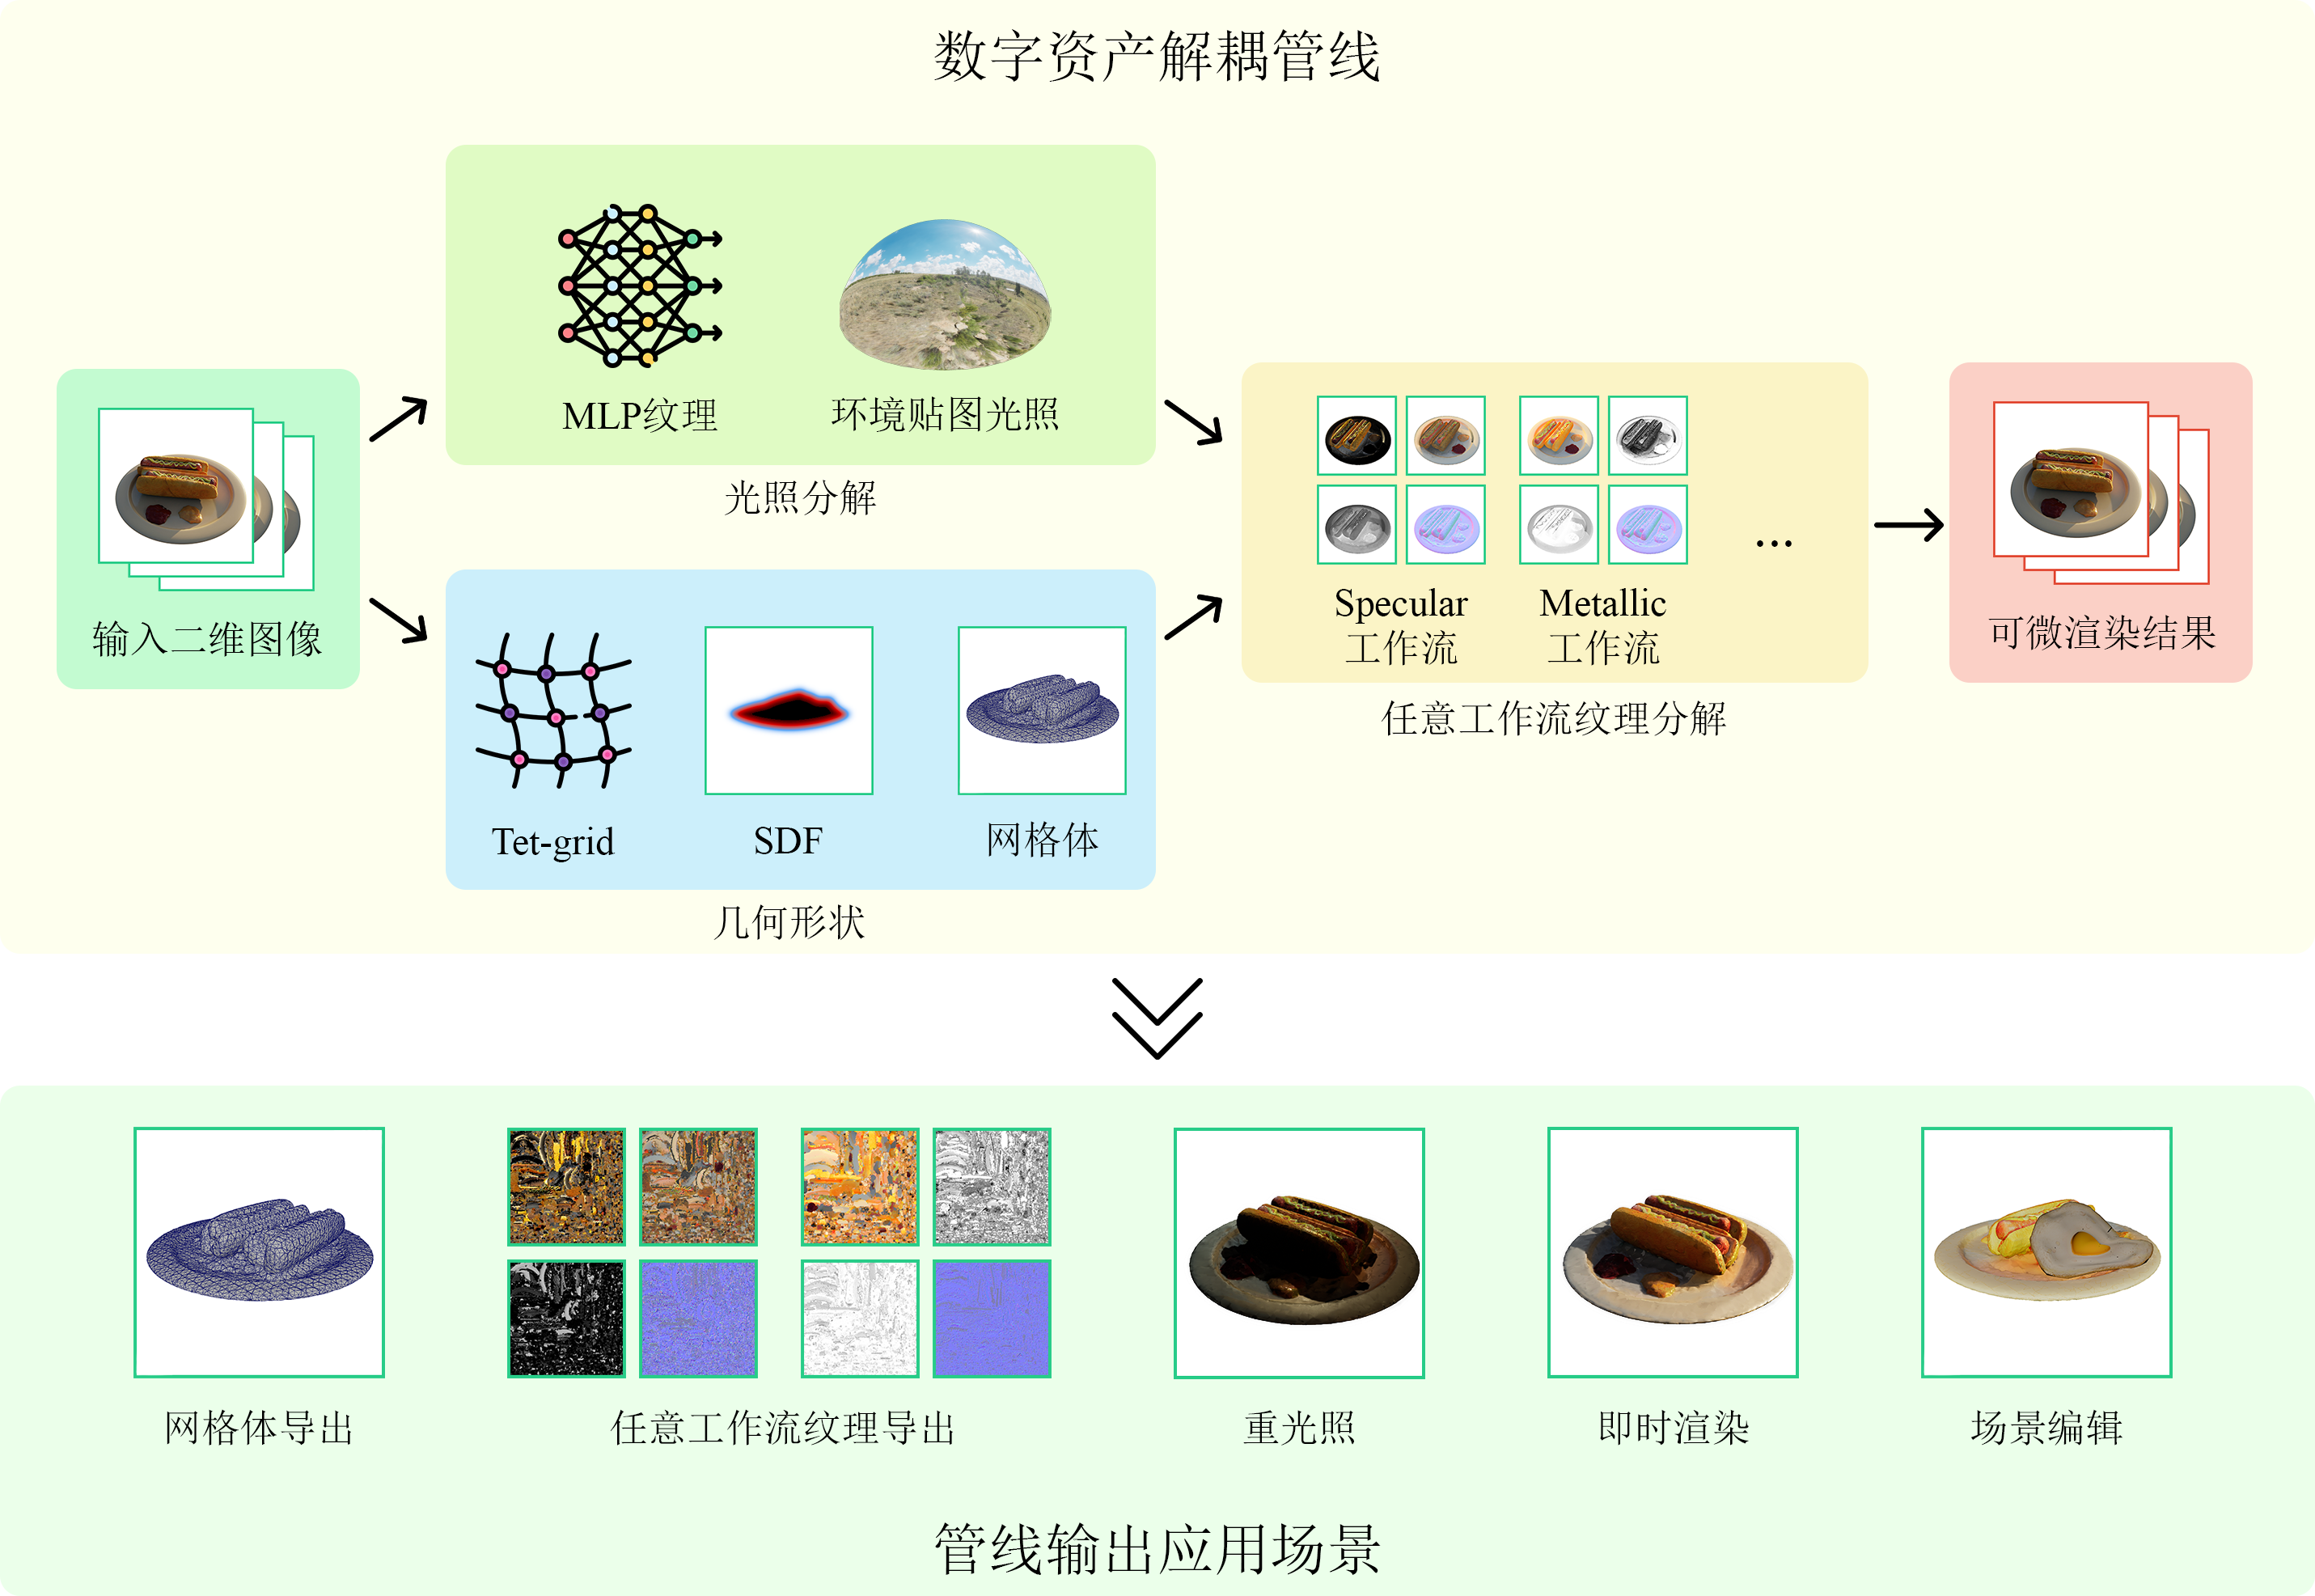
\includegraphics[width=1.0\linewidth]{Main_line_with_apply_with_big_zi.png}
  \caption{数字资产解耦管线与应用场景}
  \label{fig:main_pipe_line}
\end{figure}

\section{数字资产解耦问题分析}

工业界现有的资产大多归属于特定的工作流,而不同的着色模型也与工作流逐一对应,因此,
本文管线如果能够实现将任意工作流的数字资产转换到另一种任意工作流,即可将数字资产与任意的渲染技术相结合,
实现本文解耦的目标。

在技术路线上,本文选择了第二章中介绍的NeRF光照分解相关研究,在此基础上进行目标的实现。
NeRF光照分解管线所需的输入为场景的二维RGB图片,而待转换的数字资产可以通过渲染获得这些图片;
同时,该管线可以输出场景的几何形状和表面反射属性,与数字资产转换所需的输出类似。因此,
选择该技术开展研究和实现,对于本文的目标具备可行性。

但是,现有的工作为了提升几何重建效果,大多延续了NeRF中的隐式神经几何表示,
这导致管线的输出仅能用于重光照或新视角合成任务。而本文的目标是管线的输出能够无缝对接传统渲染器,
应用于即时渲染和下游编辑,因此本文需要对管线中的几何表示进行改造,使其输出显式网格体几何表示。
其次,现有管线受限于可微渲染的优化效率,多采用数据驱动的BRDF或固定规格的参数化BRDF作为反射属性表示,
无法满足本文使用任意工作流的需求,所以有必要针对反射属性部分重新设计,把指定工作流的纹理贴图作为输出。

基于以上分析,本文将目标进一步设置为,设计并实现一套管线,其输入为多张相机位姿已知、
光照环境及场景三维信息未知的二维RGB图片;输出为场景的几何形状和反射属性。其中,
输出的几何表示为网格体,反射属性为指定工作流对应的纹理贴图。

\section{管线设计}
本节将系统地介绍本文管线的设计与创新方法。首先,本文改进了几何表示方式,
通过一种显式隐式混合的方法,使得管线能够基于隐式表示进行优化的同时,
也能够直接输出显式网格表示的场景几何信息。随后,本文采用MLP纹理表示场景的表面反射属性,
这种设计带来了足够的灵活性,能够满足本文对任意工作流进行解耦的需求。
结合环境光照贴图作为光照技术进行可微渲染。在可微渲染中,本文允许使用任意的工作流表示
作为场景的反射属性的表示方法,使用渲染结果与原始输入计算损失,并将梯度传播到前述的几个阶段。
最后,本文管线输出网格体与纹理贴图,完成数字资产解耦的目标。接下来,本节将分别介绍以上部分。

\subsection{几何表示方式}

现有的隐式神经表示方法难以将生成结果直接用于下游编辑等任务,而传统的显式网格体则在重建效果上有所折损。
因此,本文采用了混合的几何表示方法DMTet\cite{shen2021deep},
其结合了SDF与网格体表示的优点,同时能够与传统渲染器无缝衔接。

根据本文在第二章的介绍,DMTet能够先通过SDF学习几何形状,随后以可微的方式转换为三角面网格体。
为了更高效地利用这种混合形状表示,本文进一步拓展了DMTet,引入了即时渲染中法线纹理这一技术,
在优化过程中依次使用SDF、网格体、法线纹理进行优化,接下来本文将详细介绍设计思路及实现方式。

在传统的渲染管线中,网格体在细节的精细程度取决于两个方面,首先是网格体的顶点数量,
对于细节较为丰富的区域,较高的顶点数量才能准确的还原精细结构;其次是网格体的拓扑结构,
其决定着顶点的连接和排布方式,理想的拓扑结构可以将顶点和边分配在形状发生突变的位置,
以实现相同的几何形状的同时使用尽可能少的顶点。所以,传统的数字资产在制作时通常会先完成一个较为精细的“高模”,
然后制作一个多边形数量较低的“低模”。在这一过程中,艺术家根据经验设置网格的拓扑结构,最后通过烘焙(Baking)
将“高模”中的细节以法线纹理的形式转移至“低模”中。同时,直接对网格体和法线纹理进行优化可能使得几何恢复任务变得更加困难,尤其是当凸起或凹陷既可能被网格表示,也可能被法线纹理表示时。因此,本文仅在优化的第三阶段中对法线纹理进行优化,而在前两个阶段不进行法线纹理优化。此策略能有效避免同时优化网格和法线纹理时可能出现的优化冲突问题。

基于以上这一流程,我们提出可以通过引入一个类似的逆向过程来提升几何估计的准确度,
从而改善3D重建的质量。本文设计的管线中将依次对SDF、网格体、法线纹理进行优化。首先,
SDF作为一种精细但计算效率较低的表示方式,视为“高模”,该阶段的优化目标是,发挥SDF在高频细节表示上的优势,
尽可能还原场景中的所有细节,以确保下一阶段中使用的网格具有足够的几何细节和拓扑结构。
随后,网格体的拓扑结构在经过初步的优化后将被固定,这一阶段的几何表示视为“低模”,
该优化阶段不断调整网格的顶点位置,使其精确包裹住场景的真实形状。最后,在网格体的形状确定后,
法线纹理的优化将用于表达细微的几何细节,以将场景的高频细节传递至最终网格模型中。

在具体实现中,由于SDF转换为网格体时不可避免地产生翻转或浮动的三角形面,因此本文采用了Liao等人\cite{Liao_2018}
提出的方法对DMTet的SDF值进行正则化。给定二元交叉熵损失函数$H$、Sigmoid函数$\sigma$和
符号函数$\mathrm{sign}(s_i)$,在满足$\mathrm{sign}(s_i)\neq\mathrm{sign}(s_j)$的条件下,
正则化项可以通过以下公式定义:
\begin{equation}\label{eq:Lreg}
L_{reg}=\sum_{i,j\in\mathbb{S}_e}\Bigl[H\bigl(\sigma(s_i),\mathrm{sign}(s_j)\bigr)+H\bigl(\sigma(s_j),\mathrm{sign}(s_i)\bigr)\Bigr]
\end{equation}
其中,$\mathbb{S}_e$表示四面体网格中边的集合,且条件为$\mathrm{sign}(s_i)\neq\mathrm{sign}(s_j)$。
该正则化项的直观解释是减少符号翻转的次数,从而简化表面,避免不必要的浮动几何体或内部几何结构。

随后,在对法线纹理优化的阶段中,本文没有强行固定网格体形状,但是为了避免上文所说的优化冲突问题,
本文选择使用损失函数限制法线纹理的变化,使网格体在初始化阶段保持法线纹理相对平滑,
尽可能地通过网格体形状表示场景细节。该损失函数可以由以下公式表示:

最后,本文观察到DMTet生成的网格体通常会将多个顶点挤压在一起,在局部细节上,
这有助于生成小块的平坦表面,但是在总体形状的表达上,这会导致大量的顶点和面被浪费,
无法有效表示形状。因此,本文使用如下损失函数,强制顶点之间分散开:

在后文的实验中,本文将通过定性的实验,验证该方法对于下游任务的适用性,
并通过定量的消融实验,解释并证明以上损失函数的工作原理及有效性。

\subsection{MLP纹理}
由于本文旨在使用任意工作流所对应的标准进行NeRF光照分解,因此有必要设计一种足够灵活、
易于拓展的实现方式。本文使用MLP来估计表面反射属性,以类似于体积纹理的方式建立不同的属性,
并按照通道重新划分输出用于后续的渲染步骤。

MLP整体结构如图\ref{fig:mlp_texture_cn}所示。模型首先对输入的三维坐标进行归一化处理,并利用tiny-cuda-nn框架\cite{Muller_tiny-cuda-nn_2021}
中提供的哈希网格编码器对其进行多分辨率特征映射,将输入坐标映射到高维特征空间中,增强网络对细粒度纹理信息的捕捉能力。
随后,编码器输出的特征将作为MLP的输入。MLP由一个初始全连接层,若干使用ReLU激活函数的隐藏层,以及一个输出层组成。
\begin{figure}[htb]
  \centering
  % 这里可以控制图片宽度比例
  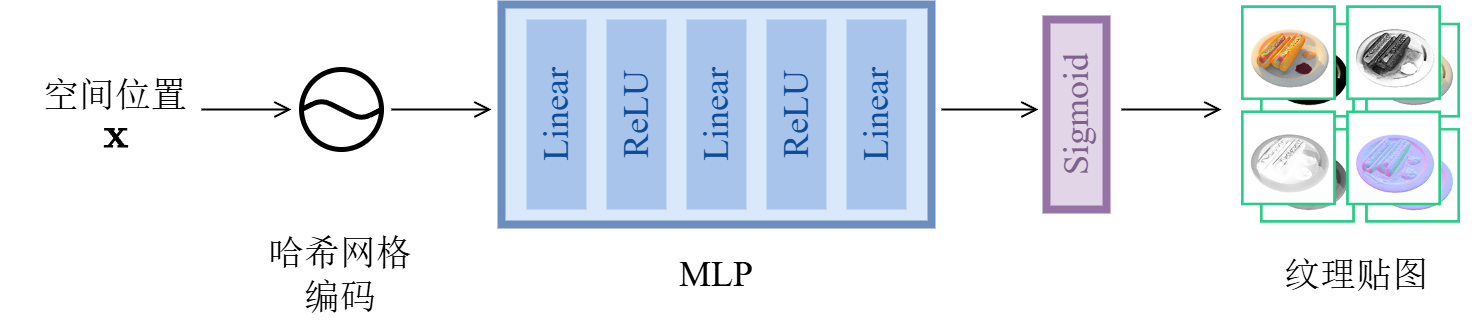
\includegraphics[width=0.8\linewidth]{MLP_texture_cn.png}
  \caption{纹理表示方式}
  \label{fig:mlp_texture_cn}
\end{figure}

由于该MLP表示的是体积纹理,因此还需要额外的采样步骤。本文首先使用xatlas生成网格体的uv坐标,随后在空间中进行采样。
在纹理导出之前,本文额外使用边缘填充算法解决了纹理的接缝问题。边缘填充算法的计算过程为算法\ref{alg:fillholes}所示:

\renewcommand{\algorithmicrequire}{\textbf{输入:}\unskip}
\renewcommand{\algorithmicensure}{\textbf{输出:}\unskip}

\begin{algorithm}
  \caption{填充空洞推拉算法}
  \label{alg:fillholes}
  \small
  \begin{algorithmic}[1]
  \REQUIRE 源图像 \texttt{src}
  \ENSURE 目标图像 \texttt{dst}
  
  \STATE 初始化图像金字塔容器 \texttt{pyramid}
  
  \STATE 创建与\texttt{src}同规格的浮点格式图像 \texttt{top}
  \STATE 将\texttt{src}拷贝至\texttt{top}
  \STATE 添加\texttt{top}到\texttt{pyramid}
  
  \WHILE{当前层宽或高 > 1}
      \STATE 获取当前层图像\texttt{big}
      \STATE $\texttt{w} \gets \max(1, \lfloor \texttt{w}/2 \rfloor)$,$\texttt{h} \gets \max(1, \lfloor \texttt{h}/2 \rfloor)$
      \STATE 创建缩小尺寸的图像 \texttt{small}
      \STATE 将\texttt{big}下采样到 \texttt{small}
      \STATE 对\texttt{small}的非零 $\alpha$ 像素执行:$\texttt{RGB} \gets \texttt{RGB} / \alpha$
      \STATE 添加\texttt{small}到\texttt{pyramid}
  \ENDWHILE
  \STATE $i \gets |pyramid| - 2$
  \WHILE{$i \textgreater 0$}
      \STATE 获取当前层图像\texttt{big}
      \STATE 创建\texttt{blowup}图像,规格与\texttt{big}相同
      \STATE 将下一层图像上采样到\texttt{blowup}
      \STATE 将\texttt{big}与\texttt{blowup}进行 $\alpha$ 合成:$\texttt{big} \gets \texttt{over}(\texttt{big}, \texttt{blowup})$
      \STATE $i \gets i - 1$
  \ENDWHILE

  \RETURN pyramid[0]
  \end{algorithmic}
  \end{algorithm}

同时,本文参照NeRFactor\cite{zhang2021nerfactor},利用损失函数对纹理的各个通道施加平滑。损失函数如下所示:

\subsection{光照表示}
本文使用第2章中介绍的IBL技术作为光照表示技术。根据\eqref{eq:rendering_equation}中的渲染方程,物体表面的出射光照
可以表示为:
\begin{equation}
  \label{eq:radiance}
  L\left(\omega_o\right)=\int_{\upOmega} L_i\left(\omega_i\right)f\left(\omega_i,\omega_o\right)\left(\omega_i\cdot\mathbf{n}\right)\mathrm{d}\omega_i,
\end{equation}
其中$L_i$表示来自方向$\omega_i$的入射辐射,$f\left(\omega_i,\omega_o\right)$为BRDF,积分域$\upOmega$为以
表面法线$\mathbf{n}$为中心的半球。由于完整的光照计算开销较高,本文使用了传统渲染引擎中常见的近似方法\cite{Hill_2014},
使用分裂和近似以进一步减少计算量。

\section{实验与结果分析}
通过前两节的分析与介绍,本文设计并实现了数字资产解耦管线,该管线能够按照任意工作流进行光照分解。为了验证
本文方法及管线的适用性和有效性,本文进行了全面的实验。接下来,本文将先介绍所用的数据集,随后进行定量实验以及定性实验,
并对实验结果进行分析。
\subsection{数据集}

为了验证本文提出的NeRF光照分解管线的有效性,我们使用公开可获取的NeRF合成数据集进行实验。
NeRF合成数据集是一个广泛使用的基准数据集,具有丰富的合成场景和高质量的图像数据,
能够充分证明本文方法在不同场景下的泛化能力。其特点包括多种复杂的场景几何形状、
不同的光照条件以及多视角的观察角度,是理想的实验数据。

其中,本文选择了4个场景,作为可视化的定性实验,随后在完整数据集上进行定量实验。
本文选择的可视化场景及理由如下:

\fourthtitle{1} Lego:
该场景包含一台由多种不同形态和颜色的积木组成的挖掘机,具有复杂的几何结构和显著的表面光泽,
可以充分验证本文管线对高频几何细节的还原能力。

\fourthtitle{2} Hotdog:
这个场景包含圆润的食物和餐具,同时具有多样的高光反射特性,对本文管线分解光泽表面的能力提出了挑战。

\fourthtitle{3} Materials:
该场景呈现了多种不同的材料,如镜面金属、磨砂金属等,每种材料具有不同的光反射属性,
能够满足验证管线识别金属或高光区域并分解的能力。

\fourthtitle{4} Mic:
该场景包括了一些微小的物体和细节,如精细结构的物体表面,并且主体材质多为磨砂金属,
可以用来验证管线在高精度要求下的适用性。

以上四个场景的预览如图\ref{fig:exp_scene}所示。

\begin{figure}[H]
  \centering
  % 这里可以控制图片宽度比例
  \begin{subfigure}[t]{0.24\textwidth}
    \centering
    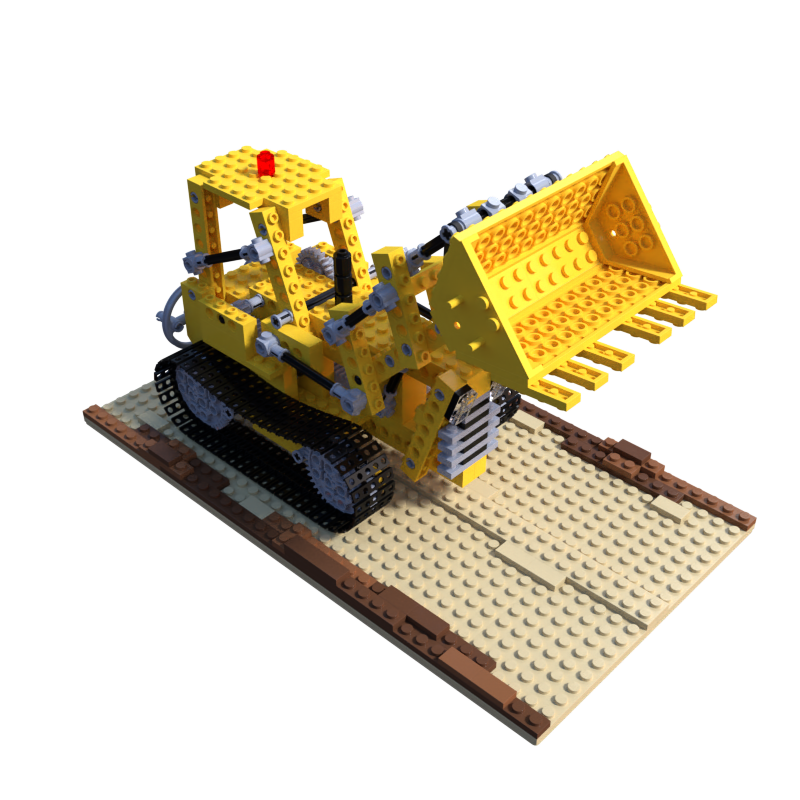
\includegraphics[width=\linewidth]{ch3/exp_scene/lego.png}
    \caption{Lego}
  \end{subfigure}
  \begin{subfigure}[t]{0.24\textwidth}
    \centering
    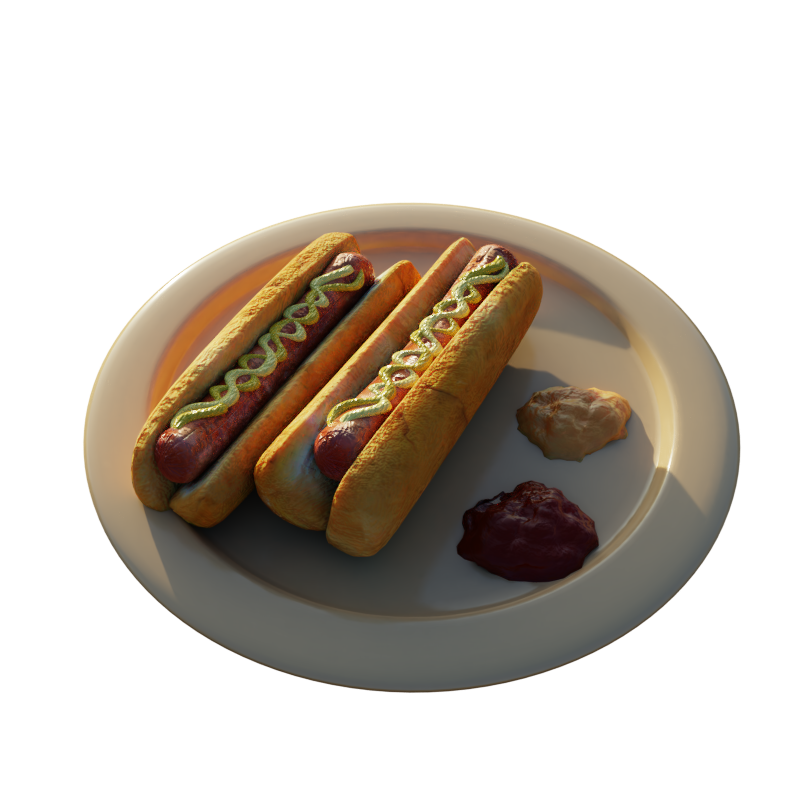
\includegraphics[width=\linewidth]{ch3/exp_scene/hotdog.png}
    \caption{Hotdog}
  \end{subfigure}
  \begin{subfigure}[t]{0.24\textwidth}
    \centering
    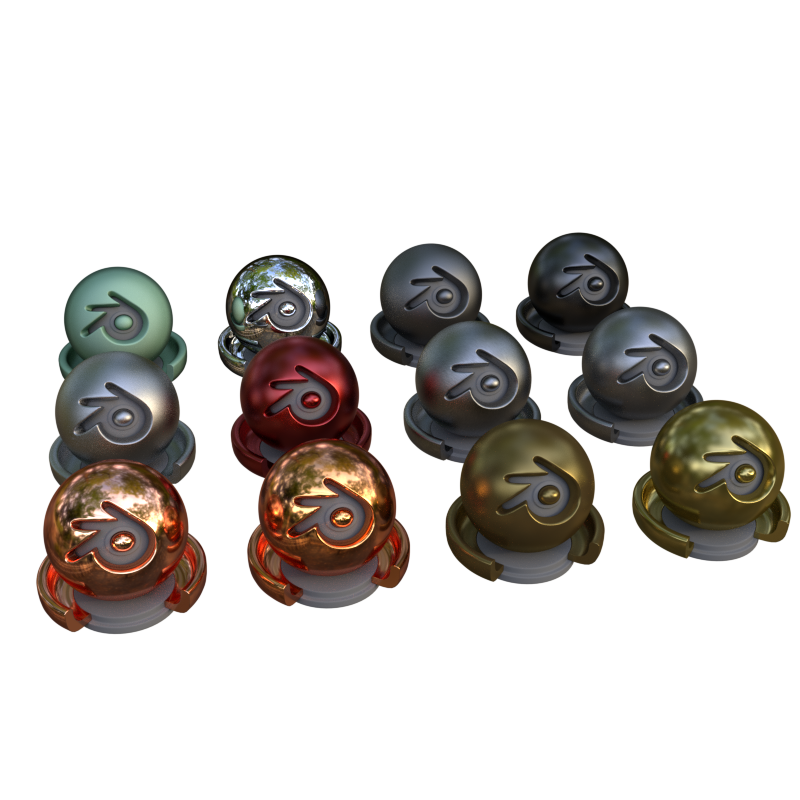
\includegraphics[width=\linewidth]{ch3/exp_scene/materials.png}
    \caption{Materials}
  \end{subfigure}
  \begin{subfigure}[t]{0.24\textwidth}
    \centering
    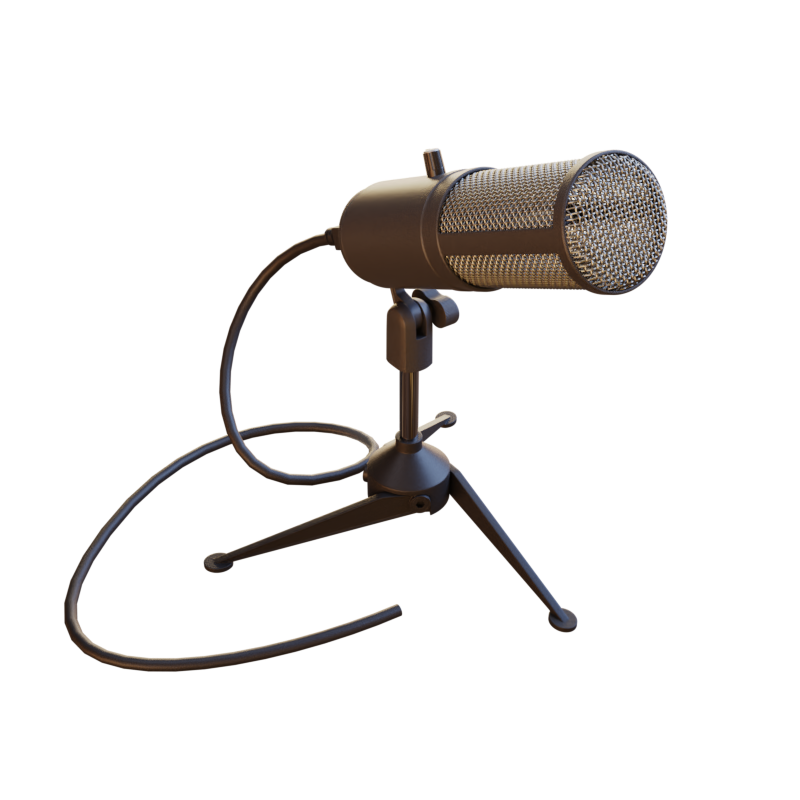
\includegraphics[width=\linewidth]{ch3/exp_scene/mic.png}
    \caption{Mic}
  \end{subfigure}
  \caption{实验场景预览}
  \label{fig:exp_scene}
\end{figure}

\subsection{多种工作流分解效果实验}
本节展示了本文提出的NeRF光照分解管线在处理任意工作流资产时的解耦效果。
在2.2.3中,我们详细介绍了3种不同的工作流,分别是Metallic工作流、Specular工作流
以及Blinn-Phong工作流。这些工作流至今仍在传统渲染引擎中得到广泛应用,
本节实验将基于这三种工作流进行分解,并展示其中4个具有代表性的不同场景可视化展示,
以定性证明本文管线能够对多种工作流进行分解。随后,本文对数据集中的全部场景进行定量比较,
分析了不同工作流对分解效果的影响。

Metallic工作流分解的实验结果如图\ref{fig:metallic_show}所示,在Metallic工作流下,
管线将输出生成Albedo、Metallic和Roughness三张纹理。在Mic和Materials场景中,
丰富的金属物体使得分解结果的特性尤为显著:Metallic纹理准确标识了金属表面区域,
充分展示了金属材料的高反射性和光泽,证明了该方法在复杂金属表面分解中的适用性。

\begin{figure}[htbp]
  \centering
  \renewcommand{\arraystretch}{1} % 调整表格行距
  \setlength{\tabcolsep}{3pt} % 调整列间距

  \begin{tabular}{c c c c c} 
      & Lego & Hotdog & Materials & Mic\\

      \raisebox{2.5\height}{\rotatebox[origin=c]{90}{Albedo}} & % 关键修改
      \subfloat{\includegraphics[width=0.22\textwidth]{ch3/metallic_show/lego/kd.png}} &
      \subfloat{\includegraphics[width=0.22\textwidth]{ch3/metallic_show/hotdog/kd.png}} &
      \subfloat{\includegraphics[width=0.22\textwidth]{ch3/metallic_show/materials/kd.png}} &
      \subfloat{\includegraphics[width=0.22\textwidth]{ch3/metallic_show/mic/kd.png}} \\

      \raisebox{2\height}{\rotatebox[origin=c]{90}{Metallic}} & % 关键修改
      \subfloat{\includegraphics[width=0.22\textwidth]{ch3/metallic_show/lego/m.png}} &
      \subfloat{\includegraphics[width=0.22\textwidth]{ch3/metallic_show/hotdog/m.png}} &
      \subfloat{\includegraphics[width=0.22\textwidth]{ch3/metallic_show/materials/m.png}} &
      \subfloat{\includegraphics[width=0.22\textwidth]{ch3/metallic_show/mic/m.png}} \\

      \raisebox{1.5\height}{\rotatebox[origin=c]{90}{Roughness}} & % 关键修改
      \subfloat{\includegraphics[width=0.22\textwidth]{ch3/metallic_show/lego/r.png}} &
      \subfloat{\includegraphics[width=0.22\textwidth]{ch3/metallic_show/hotdog/r.png}} &
      \subfloat{\includegraphics[width=0.22\textwidth]{ch3/metallic_show/materials/r.png}} &
      \subfloat{\includegraphics[width=0.22\textwidth]{ch3/metallic_show/mic/r.png}} \\

  \end{tabular}

  \caption{Metallic工作流分解效果}
  \label{fig:metallic_show}
\end{figure}

Specular工作流分解的实验结果如图\ref{fig:specular_show}所示。在Specular工作流下,管线能够同时生成Diffuse、
Specular和Glossiness三张纹理。在Hotdog场景中,光滑的盘子和粗糙的热狗被清晰地区分开来,
漫反射和镜面反射部分清晰可见,证明了该方法在Specular工作流中的适用性。

\begin{figure}[htbp]
  \centering
  \renewcommand{\arraystretch}{1} % 调整表格行距
  \setlength{\tabcolsep}{3pt} % 调整列间距

  \begin{tabular}{c c c c c} 
      & Lego & Hotdog & Materials & Mic\\

      \raisebox{2.5\height}{\rotatebox[origin=c]{90}{Diffuse}} & % 关键修改
      \subfloat{\includegraphics[width=0.22\textwidth]{ch3/specular_show/lego/diff.png}} &
      \subfloat{\includegraphics[width=0.22\textwidth]{ch3/specular_show/hotdog/diff.png}} &
      \subfloat{\includegraphics[width=0.22\textwidth]{ch3/specular_show/materials/diff.png}} &
      \subfloat{\includegraphics[width=0.22\textwidth]{ch3/specular_show/mic/diff.png}} \\

      \raisebox{2\height}{\rotatebox[origin=c]{90}{Specular}} & % 关键修改
      \subfloat{\includegraphics[width=0.22\textwidth]{ch3/specular_show/lego/spec.png}} &
      \subfloat{\includegraphics[width=0.22\textwidth]{ch3/specular_show/hotdog/spec.png}} &
      \subfloat{\includegraphics[width=0.22\textwidth]{ch3/specular_show/materials/spec.png}} &
      \subfloat{\includegraphics[width=0.22\textwidth]{ch3/specular_show/mic/spec.png}} \\

      \raisebox{1.5\height}{\rotatebox[origin=c]{90}{Glossiness}} & % 关键修改
      \subfloat{\includegraphics[width=0.22\textwidth]{ch3/specular_show/lego/gloss.png}} &
      \subfloat{\includegraphics[width=0.22\textwidth]{ch3/specular_show/hotdog/gloss.png}} &
      \subfloat{\includegraphics[width=0.22\textwidth]{ch3/specular_show/materials/gloss.png}} &
      \subfloat{\includegraphics[width=0.22\textwidth]{ch3/specular_show/mic/gloss.png}} \\

  \end{tabular}

  \caption{Specular工作流分解效果}
  \label{fig:specular_show}
\end{figure}



Blinn-Phong工作流分解的实验结果如图\ref{fig:blinn_show}所示。该工作流对应Color、Specular Roll Off和Eccentricity三张纹理。
Color纹理能够控制漫反射的基础颜色,剩余两张纹理则控制高光的形状。由于着色模型的真实感较低,
Blinn-Phong工作流漫反射颜色分解的效果显著低于其它两个工作流,无法区分明暗来自于光照还是表面固有颜色。

\begin{figure}[htbp]
  \centering
  \renewcommand{\arraystretch}{1} % 调整表格行距
  \setlength{\tabcolsep}{3pt} % 调整列间距

  \begin{tabular}{c c c c c} 
      & Lego & Hotdog & Materials & Mic\\

      \raisebox{2.7\height}{\rotatebox[origin=c]{90}{Color}} & % 关键修改
      \subfloat{\includegraphics[width=0.22\textwidth]{ch3/blinn_show/lego/kd.png}} &
      \subfloat{\includegraphics[width=0.22\textwidth]{ch3/blinn_show/hotdog/kd.png}} &
      \subfloat{\includegraphics[width=0.22\textwidth]{ch3/blinn_show/materials/kd.png}} &
      \subfloat{\includegraphics[width=0.22\textwidth]{ch3/blinn_show/mic/kd.png}} \\

      \raisebox{0.5\height}{\rotatebox[origin=c]{90}{Specular Roll Off}} & % 关键修改
      \subfloat{\includegraphics[width=0.22\textwidth]{ch3/blinn_show/lego/spec_roll.png}} &
      \subfloat{\includegraphics[width=0.22\textwidth]{ch3/blinn_show/hotdog/spec_roll.png}} &
      \subfloat{\includegraphics[width=0.22\textwidth]{ch3/blinn_show/materials/spec_roll.png}} &
      \subfloat{\includegraphics[width=0.22\textwidth]{ch3/blinn_show/mic/spec_roll.png}} \\

      \raisebox{1.5\height}{\rotatebox[origin=c]{90}{Eccentricity}} & % 关键修改
      \subfloat{\includegraphics[width=0.22\textwidth]{ch3/blinn_show/lego/ecc.png}} &
      \subfloat{\includegraphics[width=0.22\textwidth]{ch3/blinn_show/hotdog/ecc.png}} &
      \subfloat{\includegraphics[width=0.22\textwidth]{ch3/blinn_show/materials/ecc.png}} &
      \subfloat{\includegraphics[width=0.22\textwidth]{ch3/blinn_show/mic/ecc.png}} \\

  \end{tabular}

  \caption{Blinn-Phong工作流分解效果}
  \label{fig:blinn_show}
\end{figure}

表\ref{tab:rendering_comparison}展示了不同工作流解耦的对比指标,注意到部分场景在不同的工作流中出现了结果略微变化的现象,
本文认为其原因为场景特性与工作流匹配程度不同。例如,对于Lego和Hotdog场景,金属物体较少,反光物体较多,
因此在Specular工作流中表现略好;对于Materials和Mic场景,金属物体占比较多,反射更强烈,因此Metallic工作流表现更好。
另外,Metallic和Specular两种工作流效果在平均值上优于Blinn-Phong工作流,这可能是因为前二者使用了基于物理的着色模型进行渲染,
而Blinn-Phong使用的是经验模型,在渲染技术的真实感上有所不同。
\begin{table}[h]
  \centering
  \caption{不同工作流定量实验结果}
  \begin{tabular}{l ccc ccc ccc}
      \toprule
      & \multicolumn{3}{c}{Metallic} & \multicolumn{3}{c}{Specular} & \multicolumn{3}{c}{Blinn-Phong} \\
      \cmidrule(lr){2-4} \cmidrule(lr){5-7} \cmidrule(lr){8-10}
      & PSNR$\uparrow$ & LPIPS$\downarrow$ & SSIM$\uparrow$ & PSNR$\uparrow$ & LPIPS$\downarrow$ & SSIM$\uparrow$ & PSNR$\uparrow$ & LPIPS$\downarrow$ & SSIM$\uparrow$ \\
      \midrule
      Lego & 28.99 & 0.055 & 0.948 & 29.21 & 0.046 & 0.959 & 28.87 & 0.058 & 0.945 \\
      Hotdog & 33.13 & 0.047 & 0.973 & 35.78 & 0.041 & 0.979 & 31.36 & 0.065 & 0.963 \\
      Materials & 26.39 & 0.077 & 0.929 & 25.62 & 0.078 & 0.914 & 23.39 & 0.119 & 0.881 \\
      Mic & 31.01 & 0.033 & 0.976 & 29.90 & 0.037 & 0.968 & 28.85 & 0.052 & 0.960 \\
      Chair & 31.97 & 0.033 & 0.971 & 31.44 & 0.042 & 0.961 & 29.82 & 0.044 & 0.956 \\
      Drums & 24.55 & 0.078 & 0.922 & 23.61 & 0.083 & 0.910 & 23.80 & 0.082 & 0.916 \\
      Ficus & 24.68 & 0.079 & 0.932 & 24.28 & 0.082 & 0.926 & 24.18 & 0.087 & 0.923 \\
      Ship & 26.17 & 0.168 & 0.824 & 27.74 & 0.176 & 0.801 & 25.40 & 0.183 & 0.806 \\
      \midrule
      Mean & 28.36 & 0.071 & 0.934 & 28.45 & 0.073 & 0.927 & 26.96 & 0.086 & 0.919 \\
      \bottomrule
  \end{tabular}
  \label{tab:rendering_comparison}
\end{table}

实验结果显示,本文所提出的NeRF光照分解管线在处理多种传统工作流资产时表现出优异的解耦效果。
在Lego场景中,通过对复杂几何结构与多色积木构成的挖掘机进行分解,管线不仅成功捕捉到了细微的几何变化,
还精准地反映了在不同光照条件下表面光泽与材质的变化;这证明了方法在复杂结构和动态光照响应上的鲁棒性。
Hotdog场景的实验则表明,该管线能够有效分离出漫反射与镜面反射等不同光照成分,同时保持食物和餐具圆润平滑的几何细节。
Materials场景展示了其在多材质条件下的适用性,通过准确识别金属、塑料和陶瓷等不同材料的反射特性,
实现了精细几何信息的恢复。而在要求更高的Mic场景中,管线仍然能够从微小物体和复杂表面中提取出细致的几何与反射属性,
充分展示了其高效性和适应性。综上所述,这些实验结果全面验证了该方法在各类场景下实现几何与光照反射属性有效解耦的能力,
为传统渲染工作流提供了全新的高效解决方案。

\subsection{分解结果重渲染与编辑实验}

本节实验旨在评估本文提出的光照分解管线的输出结果在传统渲染器以及下游编辑任务中的应用效果。
为了检验其在实际渲染环境中的表现,我们选择了虚幻引擎5.3作为渲染器。虚幻引擎5.3是行业内主流的游戏开发引擎,
广泛用于高质量图形渲染,它支持多种工作流,能够进行离线渲染和即时渲染,且具备出色的渲染效果,
适合对光照和材质细节进行细致分析,实验环境如图\ref{fig:rerender_setup}。

\begin{figure}[htb]
  \centering
  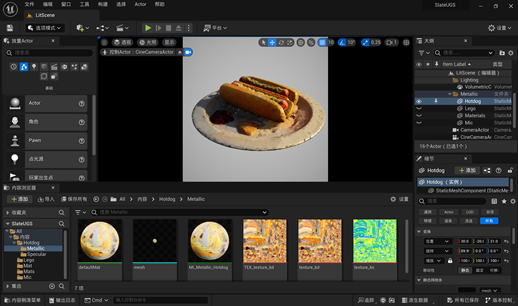
\includegraphics[width=0.8\linewidth]{ch3/rerender_setup.png}
  \caption{重渲染实验环境设置}
  \label{fig:rerender_setup}
\end{figure}

在本实验中,我们使用上一节中提到的实验结果作为数字资产,展示在虚幻引擎中的渲染效果。
每种工作流使用其对应的着色模型作为材质,进行不同视角和光照条件下的重渲染。实验结果证明了
每种工作流分解后的资产均能用于渲染,与传统数字资产具有相同的渲染效果。

其次,为了检验管线输出结果在下游编辑任务中的应用,本课题选择了Maya作为实验平台。
Maya是一款可以对网格体进行精细编辑的软件,是主流的数字资产编辑工具,
与Maya兼容可以证明本文管线输出在传统流程中的适用性。在本实验中,
本文修改了管线的输出的网格体以及贴图纹理,实验结果如图\ref{}所示。

\begin{figure}[htb]
  \centering
  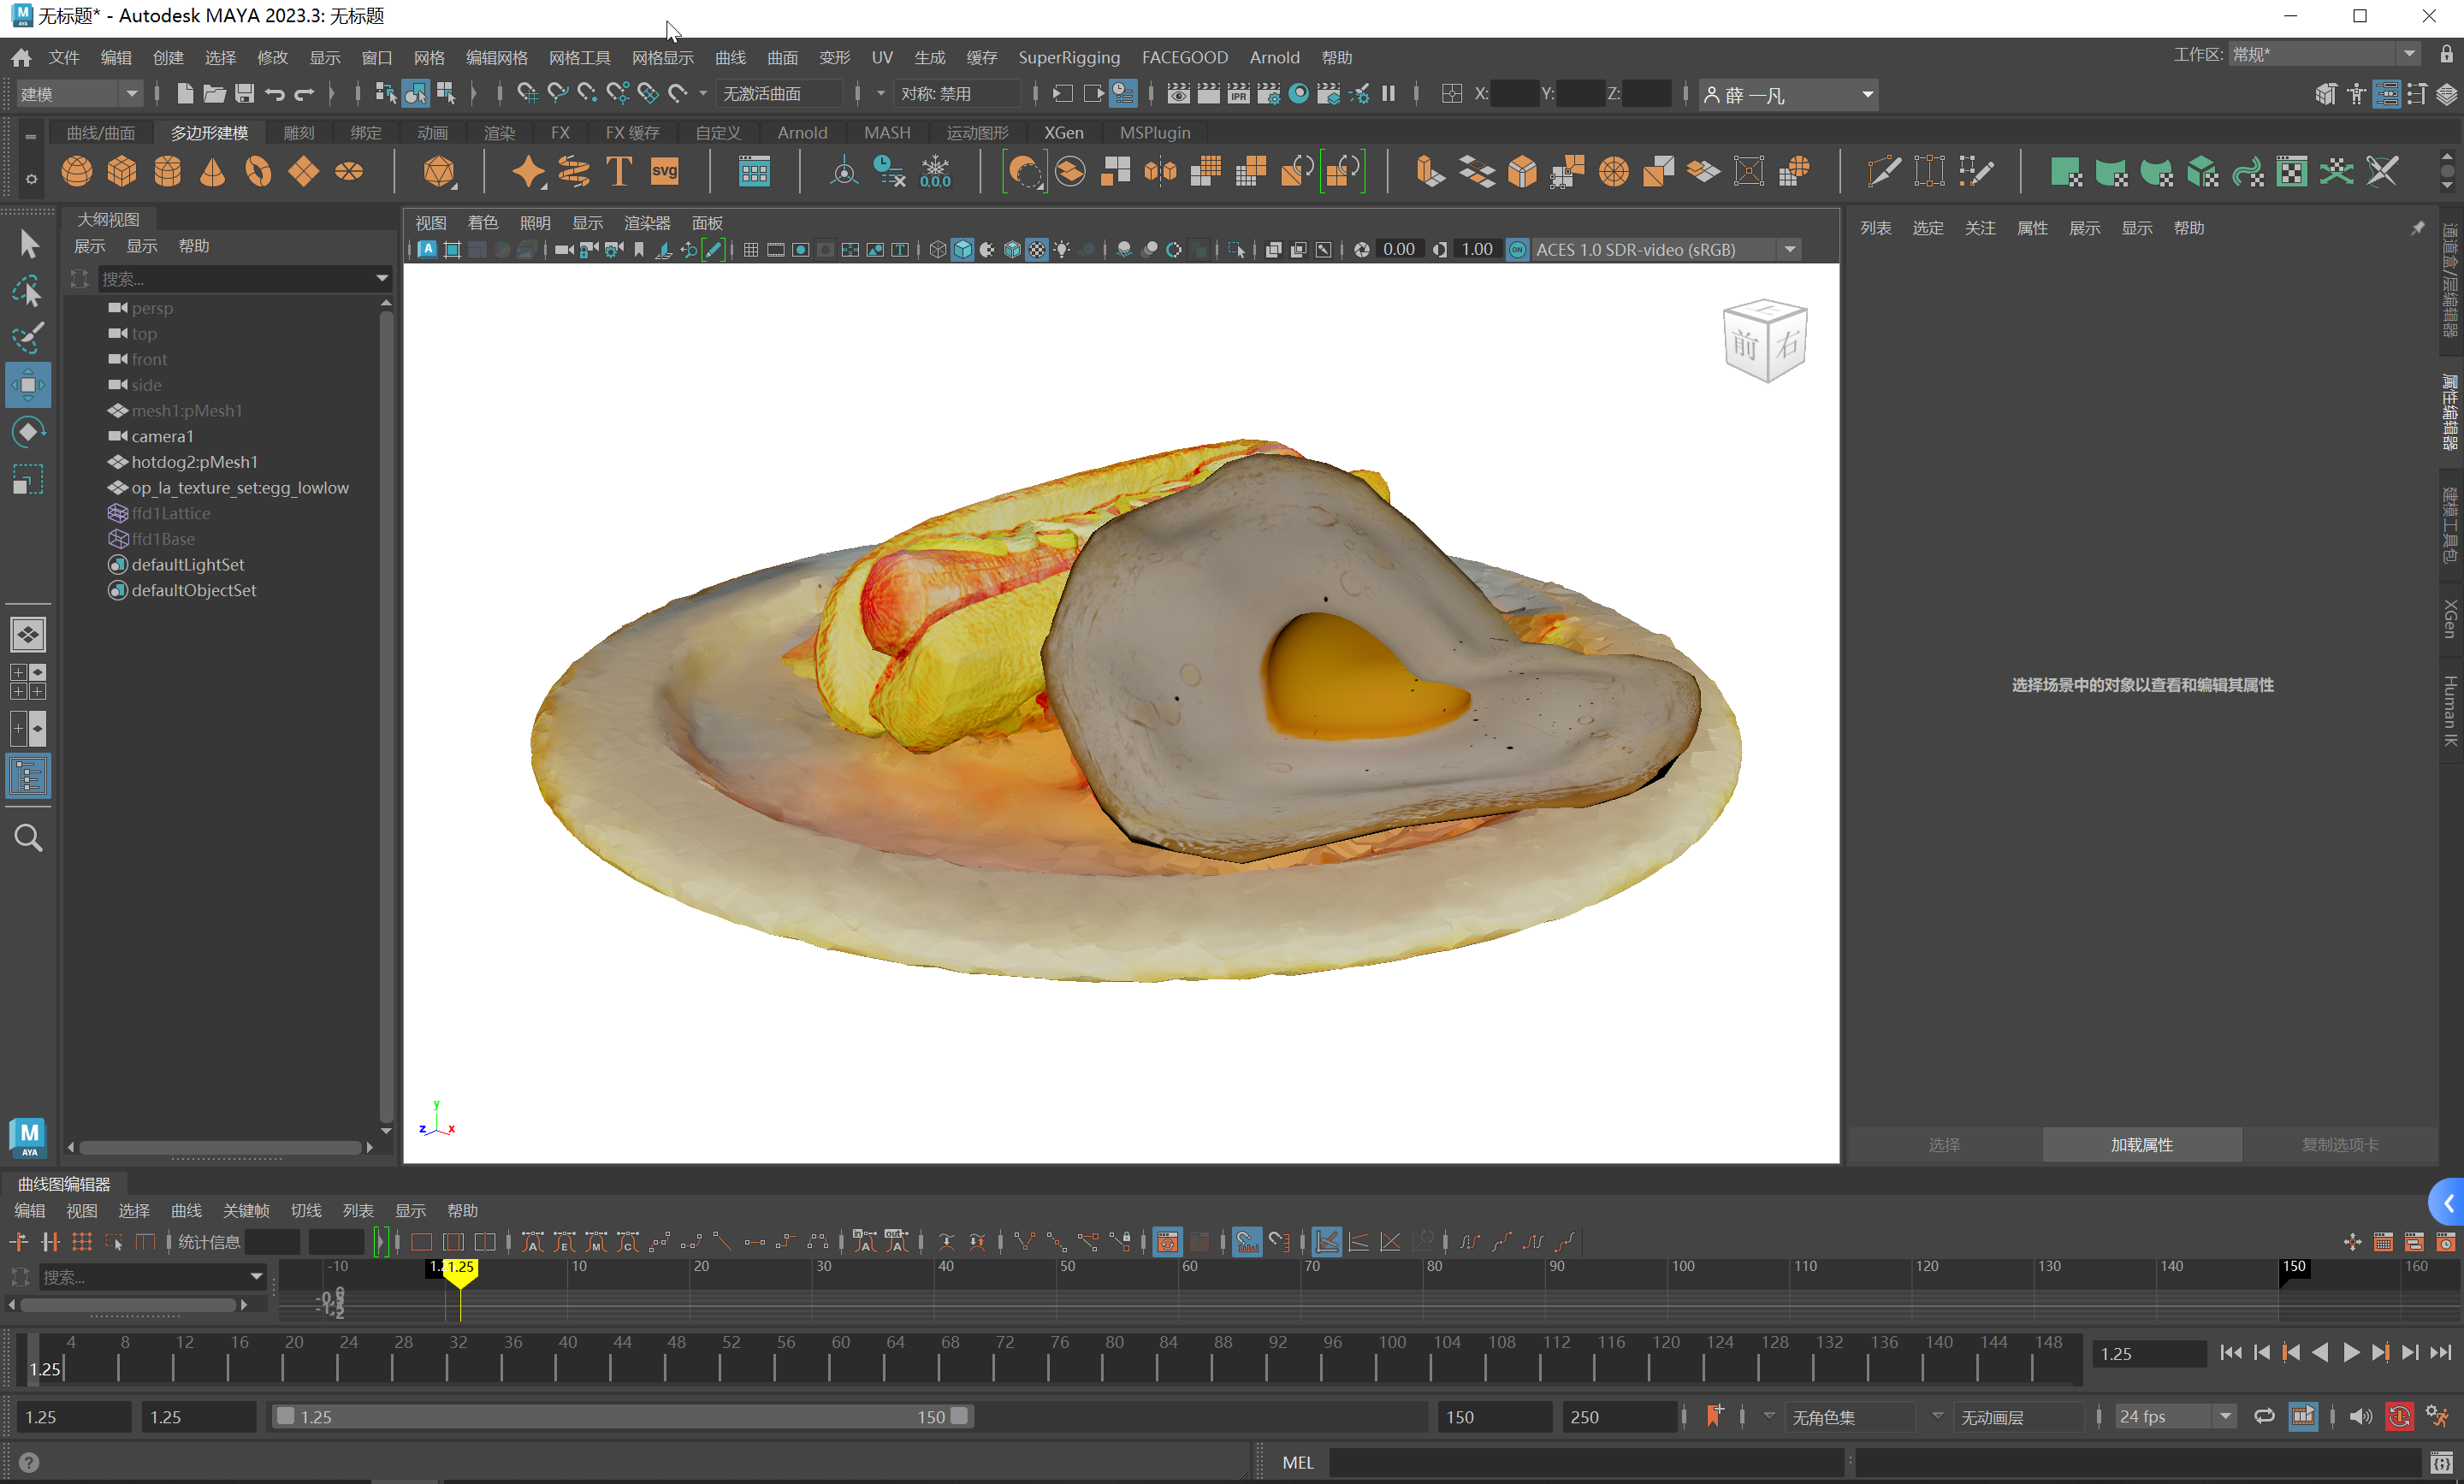
\includegraphics[width=0.8\linewidth]{ch3/maya_setup.png}
  \caption{下游编辑实验环境设置}
  \label{fig:rerender_setup}
\end{figure}

通过这些实验,本文验证了所提出的光照分解管线在传统渲染引擎中的高效性和可应用性,为后续的实际应用提供了坚实的基础。

\section{消融实验}

本节针对不同损失函数进行了定量与定性的消融实验,以证明本文设计的损失函数的有效性,并以此展示其工作原理。图\ref{fig:geo_ablation}为定性的消融实验结果,并分别展示了完整的网格体模型、网格体线框模型、局部细节三种视角。

\begin{figure}[htbp]
  \centering
  \renewcommand{\arraystretch}{1} % 调整表格行距
  \setlength{\tabcolsep}{3pt} % 调整列间距

  \begin{tabular}{c c c c} 
      \raisebox{2.5\height}{\rotatebox[origin=c]{90}{Ours}} & % 关键修改
      \subfloat{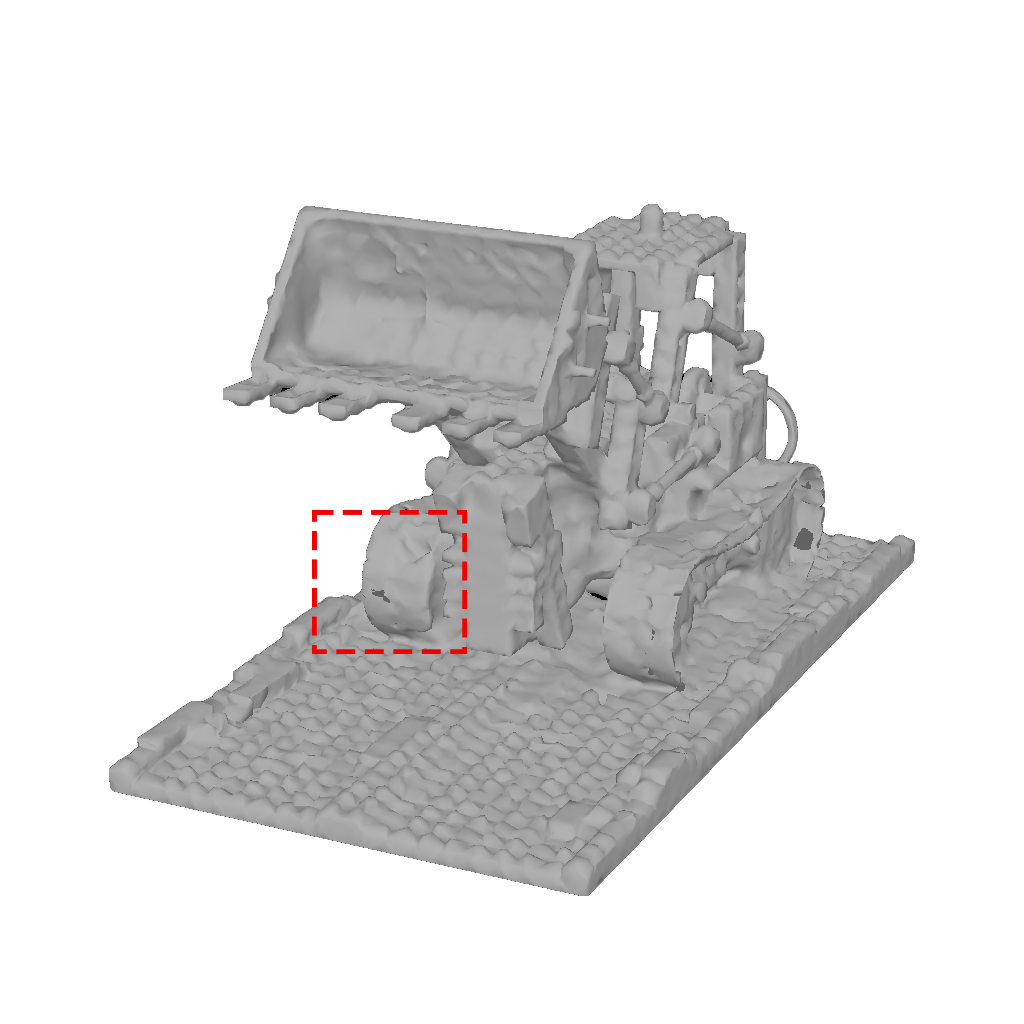
\includegraphics[width=0.3\textwidth]{ch3/geo_ablation/mesh/everything_circle.png}} &
      \subfloat{\includegraphics[width=0.3\textwidth]{ch3/geo_ablation/mesh/wo_normal.png}} &
      \subfloat{\includegraphics[width=0.3\textwidth]{ch3/geo_ablation/mesh/wo_lap.png}} \\

      \raisebox{2\height}{\rotatebox[origin=c]{90}{Ours w/o $\lambda_{\rm{normal}}$}} & % 关键修改
      \subfloat{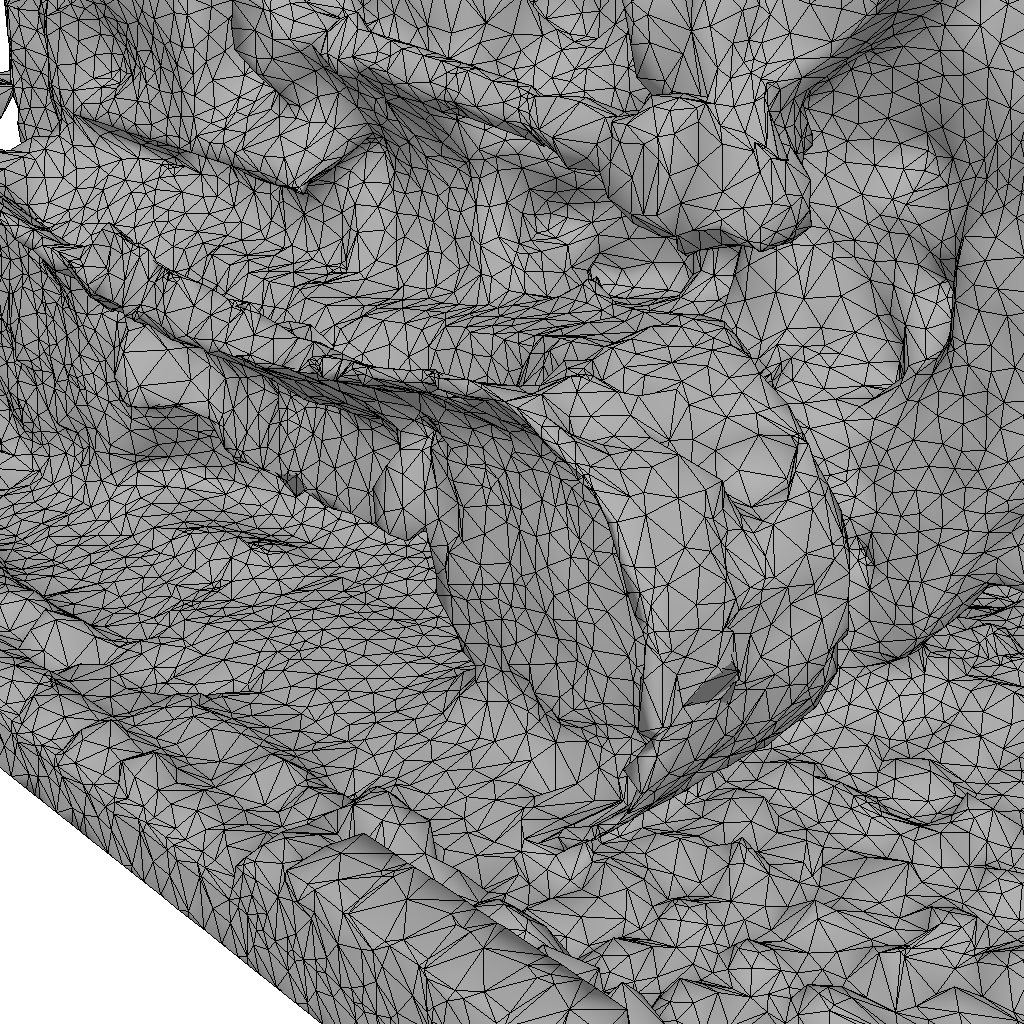
\includegraphics[width=0.3\textwidth]{ch3/geo_ablation/wired/everything.png}} &
      \subfloat{\includegraphics[width=0.3\textwidth]{ch3/geo_ablation/wired/wo_normal.png}} &
      \subfloat{\includegraphics[width=0.3\textwidth]{ch3/geo_ablation/wired/wo_lap.png}} \\

      \raisebox{1.5\height}{\rotatebox[origin=c]{90}{Ours w/o $\lambda_{\rm{laplacian}}$}} & % 关键修改
      \subfloat{\includegraphics[width=0.3\textwidth]{ch3/geo_ablation/detail/everything.png}} &
      \subfloat{\includegraphics[width=0.3\textwidth]{ch3/geo_ablation/detail/wo_normal.png}} &
      \subfloat{\includegraphics[width=0.3\textwidth]{ch3/geo_ablation/detail/wo_lap.png}} \\

  \end{tabular}

  \caption{不同损失函数的消融实验结果}
  \label{fig:geo_ablation}
\end{figure}

从线框视角能够清晰地看出,在不添加拉普拉斯平滑正则项时,可能会出现多个顶点过度聚集,以通过不正常的尖锐三角面表达高频细节。在传统渲染器中,这种结构会使得渲染结果出现不正常的突起和高光。本文认为,由于可微渲染中的渲染方式不同于传统光栅化,这样的几何结构反而不会出现视觉瑕疵,因此管线倾向于制造过于聚集的顶点分布。在添加了拉普拉斯正则项后,顶点被有效地分散开来,在总顶点数近似的情况下,能够重建更好的表面细节,同时在渲染时也避免了明显的异常瑕疵。

表\ref{tab:loss_ablation}展示了定性的实验结果。其中,加入了拉普拉斯正则化项及法线平滑正则化项的实验结果在不同指标上均有提升,也同样证明了本文方法的有效性。

\begin{table}[h]
  \centering
  \begin{tabular}{l ccc}
      \toprule
      & PSNR$\uparrow$ & LPIPS$\downarrow$ & SSIM$\uparrow$ \\
      \midrule
      Ours & 28.99 & 0.055 & 0.948 \\
      Ours w/o $\mathcal{L}_{normal}$ & 28.38 & 0.063 & 0.941 \\
      Ours w/o $\mathcal{L}_{laplacian}$ & 27.25 & 0.057 & 0.939 \\
      \bottomrule
  \end{tabular}
  \caption{不同损失函数的定量消融实验结果}
  \label{tab:loss_ablation}
\end{table}
